
% ----------------------------------------------------------------------
% Set the document class
% ----------------------------------------------------------------------
\documentclass[12pt	]{article}
\usepackage{multirow}
\usepackage{matlab-prettifier}



% ----------------------------------------------------------------------
% Define external packages, language, margins, fonts, new commands 
% and colors
% ----------------------------------------------------------------------
\usepackage[utf8]{inputenc} % Codification
\usepackage[english]{babel} % Writing idiom

\usepackage[export]{adjustbox} % Align images
\usepackage{amsmath} % Extra commands for math mode
\usepackage{amssymb} % Mathematical symbols
\usepackage{anysize} % Personalize margins
    \marginsize{2cm}{2cm}{2cm}{2cm} % {left}{right}{above}{below}
\usepackage{appendix} % Appendices
\usepackage{cancel} % Expression cancellation
\usepackage{caption} % Captions
\usepackage{listings}
\usepackage{xcolor}


    \DeclareCaptionFont{newfont}{\fontfamily{cmss}\selectfont}
    \captionsetup{labelfont={bf, newfont}}
\usepackage{cite} % Citations, like [1 - 3]
\usepackage{color} % Text coloring
\usepackage{fancyhdr} % Head note and footnote
    \pagestyle{fancy}
    \fancyhf{}
    \fancyhead[L]{\footnotesize \fontfamily{cmss}\selectfont Architecture of Network Devices} % Left of Head note
    \fancyhead[R]{\footnotesize \fontfamily{cmss}\selectfont CE5604} % Right of Head note
    \fancyfoot[L]{\footnotesize \fontfamily{cmss}\selectfont CE Dep.} % Left of Footnote
    \fancyfoot[C]{\thepage} % Center of Footnote
    \fancyfoot[R]{\footnotesize \fontfamily{cmss}\selectfont AUT} % Right of Footnote
    \renewcommand{\footrulewidth}{0.4pt} % Footnote rule
\usepackage{float} % Utilization of [H] in figures
\usepackage{graphicx} % Figures in LaTeX
\usepackage[colorlinks = true, plainpages = true, linkcolor = blue, urlcolor = blue, citecolor = blue, anchorcolor = blue]{hyperref}
\usepackage{indentfirst} % First paragraph
\usepackage[super]{nth} % Superscripts
\usepackage{siunitx} % SI units
\usepackage{subcaption} % Subfigures
\usepackage{titlesec} % Font
    \titleformat{\section}{\fontfamily{cmss}\selectfont\Large\bfseries}{\thesection}{1em}{}
    \titleformat{\subsection}{\fontfamily{cmss}\selectfont\large\bfseries}{\thesubsection}{1em}{}
    \titleformat{\subsubsection}{\fontfamily{cmss}\selectfont\normalsize\bfseries}{\thesubsubsection}{1em}{}
    \fancyfoot[C]{\fontfamily{cmss}\selectfont\thepage}

% Random text (not needed)
\usepackage{lipsum}
\usepackage{duckuments}

% New and re-newcommands
\newcommand{\sen}{\operatorname{\sen}} % Sine function definition
\newcommand{\HRule}{\rule{\linewidth}{0.5mm}} % Specific rule definition
\renewcommand{\appendixpagename}{\LARGE \fontfamily{cmss}\selectfont Appendices}

% Colors
\definecolor{istblue}{RGB}{3, 171, 230}
\definecolor{dkgreen}{rgb}{0,0.6,0}
\definecolor{gray}{rgb}{0.5,0.5,0.5}

% Image path
\graphicspath{ {./Images/} }

\usepackage[most]{tcolorbox}



% Some definitions to use color
% Default fixed font does not support bold face
\DeclareFixedFont{\ttb}{T1}{txtt}{bx}{n}{9} % for bold
\DeclareFixedFont{\ttm}{T1}{txtt}{m}{n}{9}  % for normal

% Custom colors
\usepackage{color}
\definecolor{deepblue}{rgb}{0,0,0.5}
\definecolor{deepred}{rgb}{0.6,0,0}
\definecolor{deepgreen}{rgb}{0,0.5,0}

\usepackage{listings}




\lstdefinestyle{pythonstyle}{
	language=Python,
	frame=lines,
	numbers=left,
	numberstyle=\tiny,
	basicstyle=\ttfamily\small,
	keywordstyle=\color{blue}\bfseries,
	stringstyle=\color{red},
	commentstyle=\color{green!60!black}\itshape,
	morekeywords={as, assert, async, await, class, def, del, elif, except, exec, finally, from, global, import, in, is, lambda, nonlocal, pass, raise, try, with, yield},
	morekeywords=[2]{self, cls, True, False, None},
	keywordstyle=[2]\color{orange},
	morekeywords=[3]{int, str, float, list, dict, tuple, set},
	keywordstyle=[3]\color{violet},
	morecomment=[s][\color{magenta}]{'''}{'''},
	showstringspaces=false,
	breaklines=true,
	captionpos=b,
	tabsize=2
}



%%%%%%%%%%%%%%%%%%%%%%%%%%%%%%%%%%%%%%%%%% Solution box setting %%%%%%%%%%%%%%%%%%%%%%%%%%%%%%%%%%%%%%%%%%
\newtcbtheorem{Problem}{\bfseries Problem}{enhanced,drop shadow={black!50!white},
	coltitle=black,
	top=0.3in,
	attach boxed title to top left=
	{xshift=1.5em,yshift=-\tcboxedtitleheight/2},
	boxed title style={size=small,colback=pink}
}{summary}

\newtcolorbox[auto counter]{summary}[1][]{title={\bfseries Problem~\thetcbcounter},enhanced,drop shadow={black!50!white},
	coltitle=black,
	top=0.3in,
	attach boxed title to top left=
	{xshift=1.5em,yshift=-\tcboxedtitleheight/2},
	boxed title style={size=small,colback=pink},#1}
	
%%%%%%%%%%%%%%%%%%%%%%%%%%%%%%%%%%%%%%%%%%%%%%%%%%%%%%%%%%%%%%%%%%%%%%%%
%                                 Document                             %
%%%%%%%%%%%%%%%%%%%%%%%%%%%%%%%%%%%%%%%%%%%%%%%%%%%%%%%%%%%%%%%%%%%%%%%%
\begin{document}

% ----------------------------------------------------------------------
% Cover
% ----------------------------------------------------------------------
\begin{center}
    \begin{figure}
        \vspace{-1.0cm}
        \centering
        
\includegraphics[scale = 0.35]{Images/AUT_logo.png} % IST logo
    \end{figure}
    \mbox{}\\[2.0cm]
    \textsc{\Huge \textbf{Architecture of Network Devices}}\\[1.0cm]
    \textsc{\LARGE Instructor: \href{https://scholar.google.com/citations?user=aIiC_6UAAAAJ&hl=en}{\textcolor{black}{Prof. Masoud Sabaei}}}\\[2.5cm]
    \textsc{\LARGE Amirkabir University of Technology} \\%\\[1.0cm]
    \textsc{(Tehran polytechnic)}
    \HRule\\[0.4cm]
    {\large \bf {\fontfamily{cmss}\selectfont APSARA Matching} }\\[0.2cm]
    \HRule\\[1.5cm]
\end{center}

\begin{flushleft}
    \textbf{\fontfamily{cmss}\selectfont Authors:}
\end{flushleft}

\begin{center}
    \begin{minipage}{0.5\textwidth}
        \begin{flushleft}
            \href{https://rezaadinepour.github.io/}{\textcolor{black}{Reza Adinepour}}\\
        \end{flushleft}
    \end{minipage}%
    \begin{minipage}{0.5\textwidth}
        \begin{flushright}
            \href{mailto:adinepour@aut.ac.ir}{\texttt{adinepour@aut.ac.ir}}
        \end{flushright}
    \end{minipage}
\end{center}

\vspace{1em}

    
\begin{center}
    \bigskip \bigskip \bigskip \bigskip
    \large \bf \fontfamily{cmss}\selectfont Fall 2024
\end{center}

\thispagestyle{empty}

\setcounter{page}{0}

\newpage

% ----------------------------------------------------------------------
% Contents
% ----------------------------------------------------------------------
\tableofcontents

\newpage

% ----------------------------------------------------------------------
% Body
% ----------------------------------------------------------------------

% ------------------Section 1--------------------

%\begin{figure}[h]
%	\centering
%	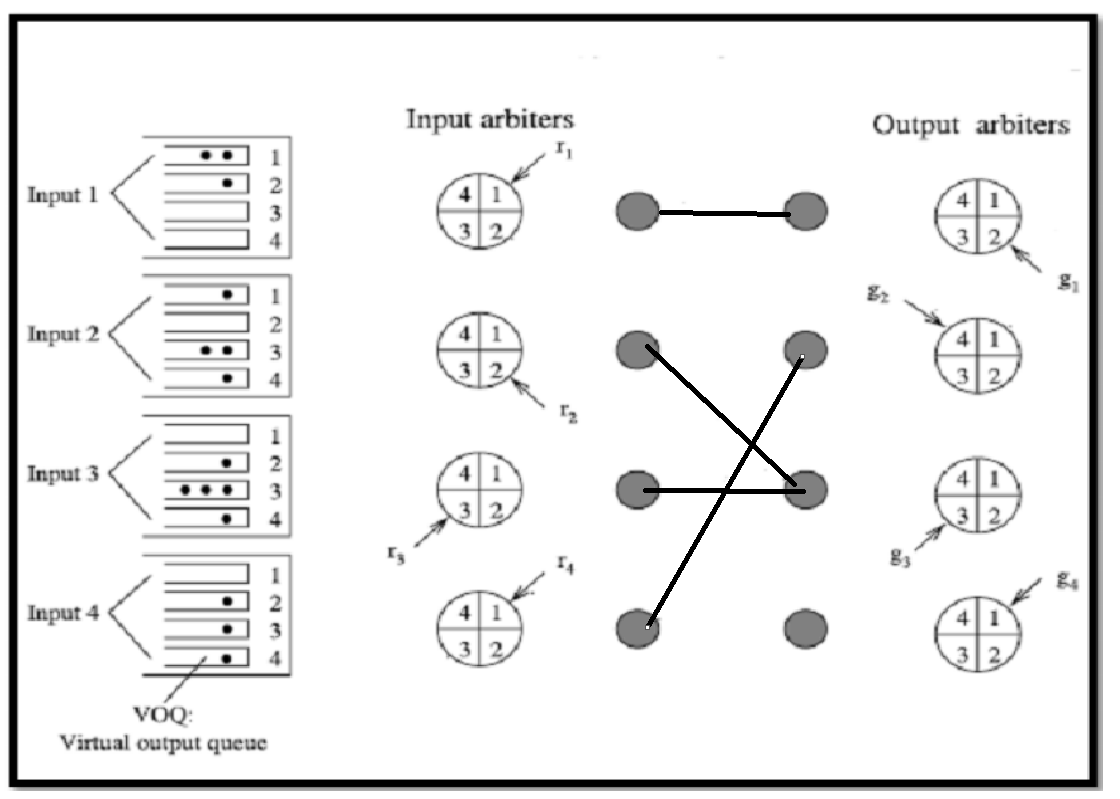
\includegraphics[width=0.8\textwidth]{Images/img6.png}
%	\caption{Overview of cyber physical systems.}
%	\label{fig:Overview of cyber physical systems}
%\end{figure}



\section{Abstract}
The APSARA algorithm \cite{giaccone2003randomized} employs the following two ideas:

\begin{enumerate}
	\item Use of memory
	\item Exploring neighbors in parallel. The neighbors are defined so that it is easy to compute them using hardware parallelism.
\end{enumerate}


\section{Introduction}
The high demand for Internet bandwidth has led to increasingly higher speed links and caused an associated demand for routers with a high aggregate switching capacity. At the highest speeds, input-queued (IQ) switches have become the architecture of choice, mainly because the memory bandwidth of their packet buffers is very low compared to that of output-queued and shared-memory architectures.


\section{APSARA}
In APSARA, the ``neighbors'' of the current match are considered as candidates of the match in the next time slot. A match $S'$ is defined as a neighbor of a match $S$ if, and only if, there are two input–output pairs in $S$, say input $i_1$ to output $j_1$ and input $i_2$ to output $j_2$, switching their connections so that in $S'$ input $i_1$ connects to output $j_2$ and $i_2$ connects to output $j_1$. All other input–output pairs are the same under $S$ and $S'$. We denote the set of all the neighbors of a match $S$ as $N(S)$. As shown in Figure \ref{fig:Example of neighbors in APSARA algorithms} \cite{giaccone2002towards}, the matching $S$ for a $3 \times 3$ switch and its three neighbors $S_1$, $S_2$, and $S_3$ are given below:



\begin{figure}[h!]
	\centering
	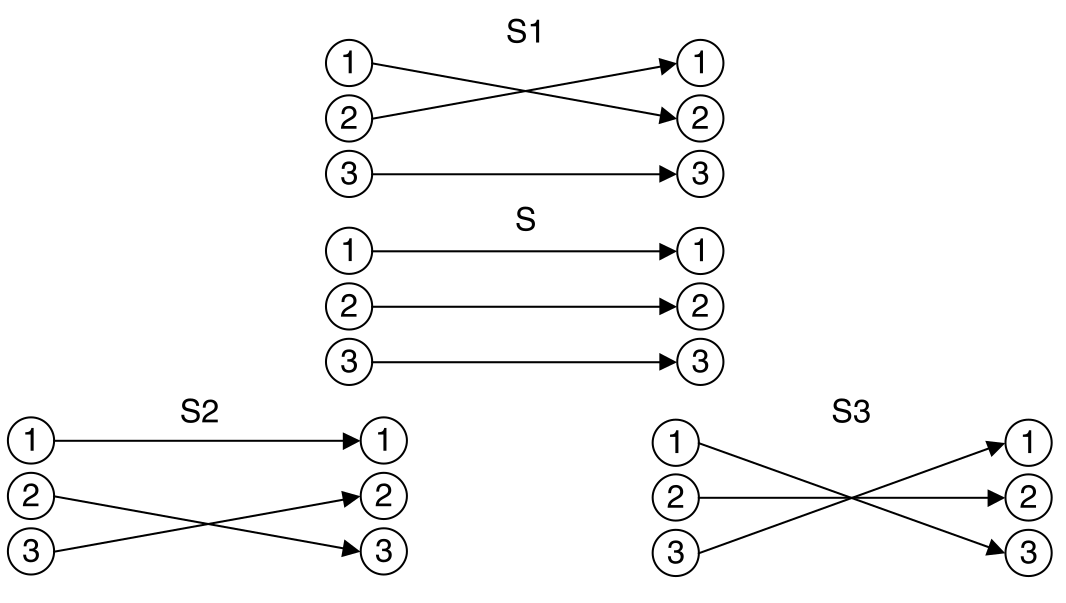
\includegraphics[width=0.8\textwidth]{Images/img5.png}
	\caption{Example of neighbors in APSARA algorithms}
	\label{fig:Example of neighbors in APSARA algorithms}
\end{figure}


\[
S = (1, 2, 3), \quad S_1 = (2, 1, 3), \quad S_2 = (1, 3, 2), \quad \text{and} \quad S_3 = (3, 2, 1).
\]


Let $S(t)$ be the matching determined by APSARA at time $t$. Let $H(t + 1)$ be the match corresponding to the Hamiltonian walk at time $t + 1$. At time $t + 1$, APSARA does the following:

\begin{enumerate}
	\item Determine $N(S(t))$ and $H(t)$.
	\item Let $M(t + 1) = N(S(t)) \cup H(t + 1) \cup S(t)$. Compute the weight $\langle S', Q(t + 1) \rangle$ for all $S' \in M(t + 1)$.
	\item Determine the match at $t + 1$ by
	\[
	S(t + 1) = \arg \max_{S' \in M(t + 1)} \langle S', Q(t + 1) \rangle. \tag{7.8}
	\]
\end{enumerate}

APSARA requires the computation of the weight of neighbors. Each such computation is easy to implement. However, computing the weights of all $\binom{N}{2}$ neighbors requires a lot of space in hardware for large values of $N$. To overcome this, two variations were considered in the work of Giaccone et al. \cite{giaccone2002towards} by reducing the number of neighbors considered in each time slot.




\section{Overview of Code Files and Functions}

This project consists of multiple files that implement the APSARA algorithm for managing input-queued switches. Below is a detailed description of each file and the functions within them.

\subsection{File: \texttt{matching.h}}
This header file defines the structure and prototypes for operations on matchings:
\begin{itemize}
	\item \texttt{struct matching}: Represents a matching configuration with:
	\begin{itemize}
		\item \texttt{n}: The number of ports.
		\item \texttt{match}: An array representing the connections between input and output ports.
	\end{itemize}
	\item \texttt{const struct matching *matching\_new(int n, const int match[])}: Allocates and initializes a new matching.
	\item \texttt{void matching\_delete(const struct matching *m)}: Frees memory allocated for a matching.
	\item \texttt{void matching\_print(const struct matching *m, FILE *fp)}: Prints the matching details to the given file pointer.
\end{itemize}

\subsection{File: \texttt{matching.c}}
This file implements the functions declared in \texttt{matching.h}:
\begin{itemize}
	\item \texttt{matching\_new}: Creates and returns a new matching structure.
	\item \texttt{matching\_delete}: Frees the memory of a matching and its internal components.
	\item \texttt{matching\_print}: Prints the input-output pairs of the matching in a formatted table.
\end{itemize}

\subsection{File: \texttt{switch.h}}
This header file defines the switch structure and its operations:
\begin{itemize}
	\item \texttt{struct sw}: Represents a switch with:
	\begin{itemize}
		\item \texttt{m}: The current matching configuration.
		\item \texttt{ports}: The number of ports.
		\item \texttt{queue}: A 2D array representing the input-output queues.
		\item \texttt{t}: The current time step.
		\item \texttt{throughput}: Tracks the total packets successfully processed.
	\end{itemize}
	\item \texttt{struct sw *switch\_new(int ports)}: Creates a new switch with the given number of ports.
	\item \texttt{void switch\_set\_current\_matching(struct sw *s, const int match[])}: Updates the current matching of the switch.
	\item \texttt{void switch\_put\_in\_queue(struct sw *s, int in\_port, int out\_port, int number)}: Adds packets to the queue for a specific input-output pair.
	\item \texttt{void switch\_process(struct sw *s)}: Processes packets based on the current matching.
	\item \texttt{void switch\_next\_matching(struct sw *s)}: Determines the next optimal matching using the APSARA algorithm.
	\item \texttt{void switch\_print(struct sw *s, FILE *fp)}: Prints the switch state to the given file pointer.
\end{itemize}

\subsection{File: \texttt{switch.c}}
This file implements the functions declared in \texttt{switch.h}:
\begin{itemize}
	\item \texttt{switch\_new}: Initializes a new switch with default matching and empty queues.
	\item \texttt{switch\_set\_current\_matching}: Updates the current matching configuration.
	\item \texttt{switch\_put\_in\_queue}: Adds packets to the appropriate queue.
	\item \texttt{switch\_process}: Processes packets based on the current matching, updating throughput and queue states.
	\item \texttt{switch\_next\_matching}: Computes the next optimal matching by considering neighbors and Hamiltonian matching.
	\item \texttt{switch\_print}: Outputs the state of the queues and matching to a log file.
\end{itemize}

\subsection{File: \texttt{permutation.h}}
Defines the permutation generation function:
\begin{itemize}
	\item \texttt{void permutation(int k, int *v, int size)}: Generates the \texttt{k}-th permutation of an array \texttt{v} of size \texttt{size}.
\end{itemize}

\subsection{File: \texttt{permutation.c}}
Implements permutation-related utilities:
\begin{itemize}
	\item \texttt{static void swap(int *v, int i, int j)}: Swaps two elements in an array.
	\item \texttt{static void next(int *v, int size)}: Computes the next permutation of the array.
	\item \texttt{permutation}: Generates the \texttt{k}-th permutation by iteratively computing the next permutation.
\end{itemize}

\subsection{File: \texttt{switch-apsara.c}}
Implements APSARA-specific functionalities:
\begin{itemize}
	\item \texttt{static const struct matching **neighbors\_matching(const struct matching *m)}: Generates all neighbors of a given matching.
	\item \texttt{static int calculate\_cost(int **queue, const struct matching *m)}: Computes the cost (number of packets served) for a matching.
	\item \texttt{static const struct matching *hamiltonian\_matching(int t, int n)}: Generates a Hamiltonian matching based on the time step \texttt{t}.
	\item \texttt{switch\_next\_matching}: Implements the core APSARA algorithm for selecting the next matching based on neighbors and Hamiltonian matching.
\end{itemize}

\subsection{File: \texttt{main.c}}
The main entry point for the simulation:
\begin{itemize}
	\item \texttt{void generate\_data(int test\_no, int ports[], int num\_ports, int load, FILE *log\_file)}: Simulates the switch operation under various conditions and logs results.
	\item \texttt{void generate\_gnuplot\_script()}: Creates a GNUplot script to visualize throughput vs. number of ports.
	\item \texttt{int main()}: The main function, responsible for running the simulation, generating data, and visualizing results.
\end{itemize}




\section{How to Run the Project}

To build and execute the project, follow these steps:

\begin{enumerate}
	\item \textbf{Create and Navigate to the Build Directory:}
	\begin{verbatim}
		$ mkdir build
		$ cd build
	\end{verbatim}
	
	\item \textbf{Generate Build Files with \texttt{cmake}:}
	\begin{verbatim}
		$ cmake ..
	\end{verbatim}
	
	\begin{figure}[h!]
		\centering
		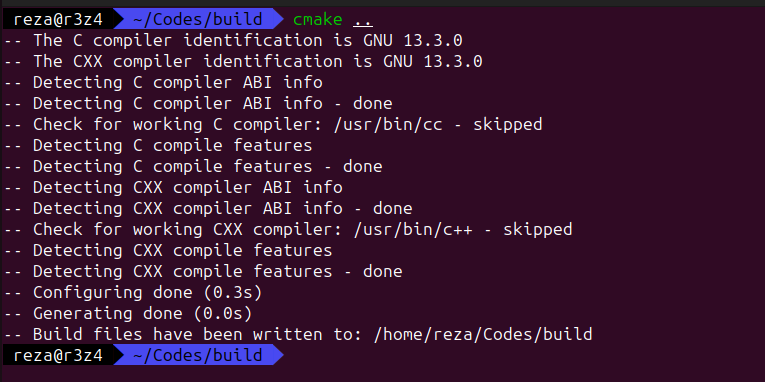
\includegraphics[width=0.8\textwidth]{Images/img1.png}
		\caption{Generate Build Files}
		\label{fig:Generate Build Files}
	\end{figure}
	
	\begin{itemize}
		\item The \texttt{cmake ..} command runs CMake in the \texttt{build} directory, specifying the parent directory (\texttt{..}) as the location of the source code.
		\item CMake generates the necessary build system files (e.g., \texttt{Makefile}) required to compile the project.
	\end{itemize}
	
	\item \textbf{Build the Project:}
	\begin{verbatim}
		$ make
	\end{verbatim}
	\newpage
	
	\begin{figure}[h!]
		\centering
		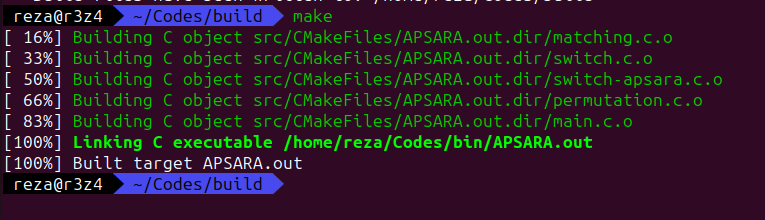
\includegraphics[width=0.8\textwidth]{Images/img2.png}
		\caption{Build the Project}
		\label{fig:Build the Project}
	\end{figure}
	
	\begin{itemize}
		\item The \texttt{make} command uses the build files generated by CMake to compile the source code.
		\item This step produces the executable file for the project, which is typically placed in the \texttt{bin} directory.
	\end{itemize}
	
	\item \textbf{Run the Program:}
	\begin{verbatim}
		$ ./../bin/APSARA.out
	\end{verbatim}
	\begin{itemize}
		\item This command executes the compiled program \texttt{APSARA.out}.
		\item The \texttt{./../bin/APSARA.out} path assumes that the executable is located in the \texttt{bin} directory relative to the \texttt{build} directory.
	\end{itemize}
	
	\begin{figure}[h!]
		\centering
		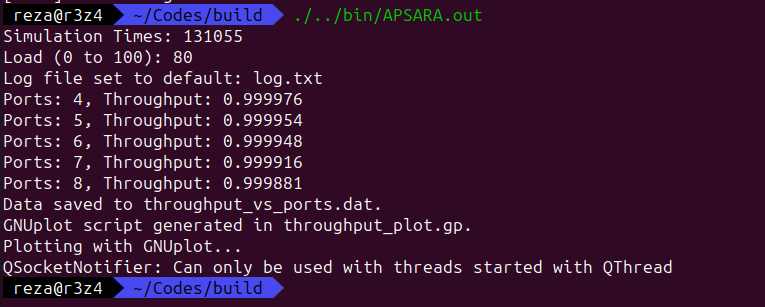
\includegraphics[width=0.8\textwidth]{Images/img4.png}
		\caption{Run Program}
		\label{fig:Run Program}
	\end{figure}
\end{enumerate}

\section{Notes}
\begin{itemize}
	\item Ensure that \texttt{CMake} and \texttt{Make} are installed on your system before running the above commands.
	\item The output and logs will be generated as specified in the \texttt{main.c} file. Review the \texttt{log.txt} file for detailed logs and \texttt{throughput\_vs\_ports.dat} for performance data.
	\item To visualize the results, the \texttt{generate\_gnuplot\_script} function creates a GNUplot script, which can be run using:
	\begin{verbatim}
		gnuplot -p throughput_plot.gp
	\end{verbatim}
	\item After running the project, the generated plots will illustrate the throughput vs. number of ports for the simulated switch.
\end{itemize}



\section{Conclusion and Results}

The simulation results, summarized in {Table~\ref{table:results}} and visualized in Figure~\ref{fig:Throughput Graph}, demonstrate that, with constant {simulation cycles} and {load}, the {throughput} decreases as the {number of ports} increases. This behavior can be explained by the following reasons:

\begin{table}[h!]
	\centering
	\caption{Simulation Results: Throughput vs. Number of Ports}
	\label{table:results}
	\begin{tabular}{||c c c c||}
		\hline
		\textbf{Port} & \textbf{Throughput} & \textbf{Load} & \textbf{Simulation Cycles} \\\hline\hline
		4 & 0.999976 & 0.80 & 131055 \\ 
		5 & 0.999954 & 0.80 & 131055 \\ 
		6 & 0.999948 & 0.80 & 131055 \\ 
		7 & 0.999916 & 0.80 & 131055 \\ 
		8 & 0.999881 & 0.80 & 131055 \\ \hline
	\end{tabular}
\end{table}



\begin{enumerate}
	\item \textbf{Increased Contention for Output Ports:}
	\begin{itemize}
		\item As the number of ports grows, more input ports attempt to connect to the available output ports, increasing the likelihood of multiple input ports competing for the same output port.
		\item When such contention occurs, only one connection can be matched at a time, leaving other packets unprocessed, as reflected in the decreasing throughput values in {Table~\ref{table:results}}.
	\end{itemize}
	
	\item \textbf{Higher Matching Complexity:}
	\begin{itemize}
		\item The APSARA algorithm evaluates neighbors to select the optimal matching at each step. As the number of ports increases, the number of possible neighbors grows exponentially, complicating the decision-making process.
		\item This complexity can result in suboptimal matching decisions within the constraints of the simulation cycles, contributing to the decline in throughput as shown in {Figure~\ref{fig:Throughput Graph}}.
	\end{itemize}
	
	\item \textbf{Queue Saturation:}
	\begin{itemize}
		\item With more ports, the system's queue capacity for each input-output pair may become limited relative to the number of packets being generated.
		\item This can result in packets waiting longer in queues, causing delays and reducing effective throughput, which is evident from the trend in both {Table~\ref{table:results}} and {Figure~\ref{fig:Throughput Graph}}.
	\end{itemize}
	
	\item \textbf{Fixed Simulation Cycles:}
	\begin{itemize}
		\item The simulation is conducted over a fixed number of cycles. As the number of ports increases, the matching process must handle more input-output combinations within the same cycles.
		\item This results in fewer overall packets being served, contributing to the observed trend in {Figure~\ref{fig:Throughput Graph}}.
	\end{itemize}
	
	\item \textbf{Increased Load Distribution:}
	\begin{itemize}
		\item For the same load percentage (e.g., 80\%), the total number of packets increases with the number of ports. However, the system's ability to process these packets does not scale proportionally due to limitations in the matching algorithm and hardware resources.
		\item This imbalance leads to reduced throughput efficiency, as indicated in the throughput values in {Table~\ref{table:results}} and the declining curve in {Figure~\ref{fig:Throughput Graph}}.
	\end{itemize}
\end{enumerate}

\begin{figure}[h!]
	\centering
	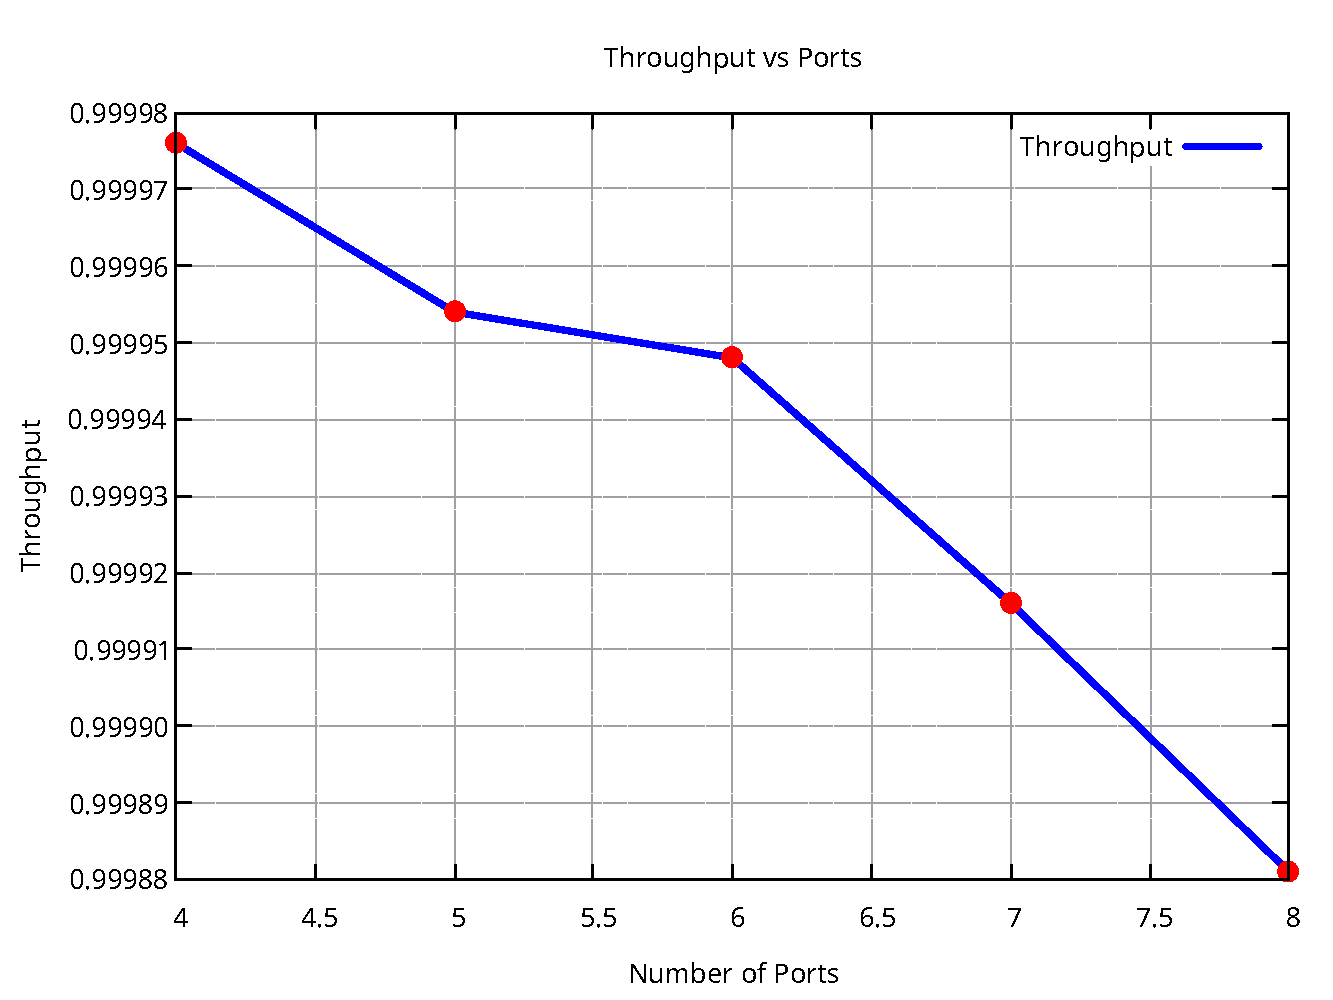
\includegraphics[width=0.85\textwidth]{Images/result.pdf}
	\caption{Throughput Graph}
	\label{fig:Throughput Graph}
\end{figure}

\section{Key Insight}

This behavior, illustrated in both {Table~\ref{table:results}} and {Figure~\ref{fig:Throughput Graph}}, highlights a fundamental trade-off in input-queued switch architectures: while adding more ports increases the switch's connectivity and capacity, it also introduces inefficiencies due to contention, complexity, and resource limitations. Advanced scheduling algorithms or additional resources, such as larger queues or faster matching processes, would be required to mitigate the decrease in throughput as the number of ports increases.











%\begin{lstlisting}[style=pythonstyle, caption={Insert Command}]
%def insert(root, prefix, length, next_hop, stride, base):
%	current_node = root  
%	integer_prefix = int(prefix[:length],base)
%	binary_number = bin(integer_prefix)[2:]
%	
%	rjusted = binary_number.rjust(length, '0')
%	binary_prefix = rjusted.ljust(32, '0')
%	
%	for i in range(0, length, stride):
%		bit_pattern = binary_prefix[i:i+stride]
%		if i + stride > length:
%			curr_pattern = str(binary_prefix[i:length]) 
%			ex = len(curr_pattern)
%			remaining_bits = stride - (length - i)
%			# Calculate the number of combinations for the remaining bits
%			num_combinations = 2 ** (remaining_bits)
%			# Generate all combinations for the remaining bits and create nodes
%			for j in range(num_combinations):
%				# Generate the binary representation for the current combination
%				combination = bin(j)[2:].zfill(remaining_bits)
%				
%				pattern = curr_pattern + combination 
%				if pattern not in current_node.children:
%					current_node.children[pattern] = Node(next_hop=next_hop, length= length)
%				else:
%					if current_node.children[pattern].length < length:
%						current_node.children[pattern].next_hop = next_hop
%						current_node.children[pattern].length = length
%		else:
%			# If there is no child for the bit pattern, create a new node
%			if bit_pattern not in current_node.children:
%				current_node.children[bit_pattern] = Node()
%			current_node = current_node.children[bit_pattern]
%			# If we have reached the end of the prefix, set the next hop
%			
%		if (i + stride == length ):
%			current_node.next_hop = next_hop
%			current_node.length = length
%\end{lstlisting}




\newpage
% ----------------------------------------------------------------------
% References
% ----------------------------------------------------------------------
\bibliographystyle{plain}
\bibliography{refs}

\end{document}